\documentclass[12pt,a4paper,italian,twoside, openany]{book}

% Set up data, if you need to add a package, go here
%
\usepackage[utf8]{inputenc}
\usepackage[T1]{fontenc}
\usepackage{graphicx}
\usepackage[nottoc]{tocbibind}
\usepackage{booktabs}
\usepackage[margin=1.5in]{geometry}
\usepackage[italian]{babel}
\usepackage{algorithm}
%\usepackage{arevmath}     % For math symbols
\usepackage[noend]{algpseudocode}
\usepackage{multirow}
\usepackage{mathtools}
\usepackage[normalem]{ulem}
\useunder{\uline}{\ul}{}
\usepackage{wrapfig}
\usepackage{todonotes}
\usepackage{adjustbox}
%\usepackage{fixltx2e}
\usepackage{caption}
\usepackage{array}
\usepackage[hidelinks]{hyperref}

\hypersetup{}
\newcolumntype{P}[1]{>{\centering\arraybackslash}p{#1}}

\usepackage[square,numbers]{natbib}
\makeatletter
\renewcommand\bibsection%
{
  \section*{\refname
    \@mkboth{\MakeUppercase{\refname}}{\MakeUppercase{\refname}}}
}
\makeatother
%%%%%%

\usepackage{xcolor}

\definecolor{codegreen}{rgb}{0,0.6,0}
\definecolor{codegray}{rgb}{0.5,0.5,0.5}
\definecolor{codepurple}{rgb}{0.58,0,0.82}
\definecolor{backcolour}{rgb}{0.95,0.95,0.92}



% macro
\newcommand{\matchNews}[1]{\emph{$news\_match$}\textsubscript{\texttt{\lowercase{#1}}}}
\newcommand{\matchRatio}[1]{\emph{$match\_ratio_{#1}$}}

\begin{document}

% viene caricato il logo vettoriale UFFICIALE dell'università
%\begin{spacing}{0.90}
\begin{center}
    {\Large \thispagestyle{empty}}{\includegraphics[scale=0.1]{images/logo.png}}\par
\end{center}
%\end{spacing}

\noindent 
\begin{center}
    \textbf{\Large Università degli Studi di Cagliari}%\par
\end{center}%{\LARGE \par}
\vspace{-1em}
\noindent 
\begin{center}
    \textbf{\large Facoltà di Scienze}\par
\end{center}{\large \par}
\vspace{-1em}
\noindent
\begin{center}
    {\large Corso di Laurea Triennale in Informatica}\par
\end{center}{\large \par}

\vspace{7em}

\noindent
\begin{center}
    \textbf{\Large Misura di posizione e velocità}\par
    \vspace{0.6em}
    \textbf{\Large in sistemi di sorveglianza stradale}\par
\end{center}{\LARGE \par}

%\begin{spacing}{0.90}
\vspace{4cm}
\textbf{\large Relatore:}{\large \hfill{}}\textbf{\large Candidato:}{\large \par}
%\end{spacing}

{\large Dott. Alessandro Sebastian Podda \hfill{}Nicola Sansoni~}{\large \par}
\vspace{1cm}
\textbf{\large Co-Relatore:}{\large \par}
{\large Prof. Salvatore M. Carta}

\vspace{2cm}

\begin{center}
    {\large ACADEMIC YEAR 2020/2021}{\large \par}
\end{center}


% ----------------------------- ABSTRACT ------------------------------------
\setlength{\parskip}{\bigskipamount}
\renewcommand{\baselinestretch}{1.4}\normalsize
\chapter*{Abstract}
Data l'alta diffusione di sistemi di video sorveglianza a camera fissa (CCTV) risulta interessante lo sviluppo di sistemi in grado di individuare, tracciare e monitorare le entità inquadrate da tale camera.
Le misure estratte dall'immagine, come posizione e velocità, risultano però distorte rispetto alla realtà. 
Questa distorsione è legata alla posizione e alla rotazione della camera rispetto alla scena inquadrata.
Chiamiamo questa distorsione \emph{distorsione prospettica}.
Lo scopo di questa tesi è quello di presentare un algoritmo di correzione della \emph{distorsione prospettica} e una metodologia interattiva per la generazione delle informazioni necessarie a tale algoritmo.


% ------------------------------- INDICE ---------------------------------------
\renewcommand{\baselinestretch}{1}\normalsize


\frontmatter 						% numerazione romana
\tableofcontents

\pagestyle{plain}
%\makeheadrule{headings}{\textwidth}{0.3pt}

\renewcommand{\baselinestretch}{1.4}\normalsize

\mainmatter
\chapter{Introduzione e stato dell'arte}
\label{sec:introduzione}

La correzione della \emph{distorsione prospettica} è un passaggio necessario nella maggioranza dei processi che estraggono informazioni da immagini acquisite attraverso una camera.
Nei casi in cui tale distorsione sia poco accentuata è possibile approssimare una correzione utilizzando trasformazioni lineari come rotazione, scalatura e shear dell'immagine.
% Negli altri casi risulta necessario un approccio più profondo, che richiede un cambio di coordinate da cartesiane a proiettive omogenee e la generazione di una matrice omografica che trasformi lo \emph{spazio immagine} in \emph{spazio reale}.
% Spesso per semplicità si riduce lo \emph{spazio reale} ad un piano approssimabile alla superficie dell'oggetto di interesse.
Negli altri casi risulta necessario un approccio più profondo: si limita lo \emph{spazio reale} preso in considerazione a un piano bidimensionale e si individua la trasformazione che proietta lo \emph{spazio immagine} nel piano scelto.
Tale trasformazione è rappresentata attraverso una matrice omografica in coordinate omogenee.
Lo studio di come generare la matrice di trasformazione in questione è esplorato in modo particolarmente esteso nel campo del processing di documenti; i documenti presentano caratteristiche facilemente individuabili su cui poter fare leva per ricavare informazioni sulla distorsione dell'immagine.
È infatti possibile sfruttare le linee parallele e perpendicolari nei bordi e nel testo per ricavare la matrice di trasformazione desiderata \cite{persp:docs}.
Un possibile approccio nel campo della video sorveglianza è quello di sfruttare un dispositivo di acquisizione immagini in grado di identificare la profondità di ogni pixel dell'immagine inquadrata e con questa ricavare la trasformazione voluta \cite{persp:depth}.
Un'ulteriore alternativa è quella di individuare una corrispondenza tra 4 punti conosciuti nello \emph{spazio reale} e nello \emph{spazio immagine} e utilizzare tale corrispondenza per generare la matrice omografica \cite{persp:map}.
% Quest'ultimo metodo è spesso utilizzato anche quando non si conoscono esattamente le coordinate dei punti nello \emph{spazio reale}, ma si conosce la loro disposizione. Individuando 4 punti che nello \emph{spazio reale} delineano un quadrato e correlandoli con i corrispettivi 4 punti nello \emph{spazio immagine} è possibile generare facilmente una matrice di correzione. Tale matrice non garantisce però magnitudini corrette e corregge solamente angoli e rapporto tra gli assi.

Nonostante tutti i metodi sopra siano ottime soluzioni, nessuna di queste è facilmente applicabile senza enormi sforzi: il metodo della mappatura richiede la conoscenza di misurazioni precise per ogni camera implementata nel sistema; il metodo della derivazione dalla profondità richiede la spesa per l'acquisto di camere in grado di rilevarla; i metodi che utilizzano linee parallele e perpendicolari, utilizzati per i documenti, sono probabilmente i più interessanti ma richiedono un enorme sforzo implementativo per essere applicati al nostro contesto.

\section{Contesto e motivazioni}

Lo sviluppo di un sistema di rilevazione di anomalie stradali richiede la conoscenza dei dati relativi alle entità presenti nella scena inquadrata dalla telecamera di sorveglianza.
In particolare risultano necessari i dati relativi a posizione, velocità e categoria delle entità.
La posizione e la categoria possono essere ricavate utilizzando una \emph{Convolutional Neural Network (CNN)} che esegue l'\emph{Object Detection}.
La velocità può poi essere ricavata applicando un algoritmo di tracciamento ai dati ottenuti nella fase di categorizzazione.

Questi dati sono però in \emph{spazio immagine} e non in \emph{spazio reale}.
Questi due spazi differiscono in numero di dimensioni, essendo lo \emph{spazio immagine} bidimensionale e lo \emph{spazio reale} tridimensionale.
Non esiste perciò una trasformazione lineare dall'uno all'altro.
Utilizzare le misurazioni in \emph{spazio immagine} per la rilevazione di anomalie porta a un sistema fragile e poco affidabile, in quanto tali misurazioni risultano distorte rispetto a i loro valori reali.

È perciò necessario individuare una trasformazione da \emph{spazio immagine} a \emph{spazio reale}.
Deve essere possibile arrivare a tale trasformazione senza conoscere i dati reali relativi alla camera e alla superficie inquadrata, in quanto questi non sono sempre disponibili.
Inoltre applicare questa trasformazione deve necessariamente essere poco costoso computazionalmente, in modo da mantenere il sistema di rilevazione di anomalie eseguibile in real time.

\section{Obiettivo della tesi}
\begin{itemize}
	\item Sviluppare un algoritmo di correzione prospettica applicabile ad un sistema di rilevazione di anomalie nel contesto della sicurezza stradale.
	\item Sviluppare e implementare un tool interattivo per la generazione di dati relativi alla distorsione prospettica della singola camera.
\end{itemize}

\section{Attività della tesi}

\begin{itemize}
	\item Studio delle trasformazioni di proiezione
	\item Sviluppo del tool interattivo per la generazione delle informazioni relative alla camera
	\item Implementazione del modulo di correzione nel sistema real time di rilevazione anomalie
	\item Confronto tra risultati con e senza correzione
\end{itemize}

\section{Schema della tesi}

Nel capitolo \ref{sec:teoria} è illustrato il problema ed è modellato dal punto di vista matematico. In questo capitolo vengono discusse e giustificate le formule applicate.

Nel capitolo \ref{sec:funzionalita} sono illustrate le funzionalità richieste ai due sistemi, quello di correzione e quello di generazione della trasformazione correttiva, e sono discusse le scelte compiute per ottenerle.

Nel capitolo \ref{sec:implementazione} è descritta brevemente l'architettura del sistema con cui il modulo di correzione interagisce e sono discusse le tecnologie e le metodologie implementative utilizzate.

Nel capitolo \ref{sec:testing} è descritto il processo di validazione e valutazione della soluzione proposta e i suoi risultati.

Infine nel capitolo \ref{sec:conclusioni} è riassunto il lavoro svolto, sono discussi i risultati ottenuti e sono suggeriti possibili sviluppi e miglioramenti,

\chapter{Funzionalità}
\label{sec:funzionalita}

Il sistema da noi sviluppato per monitorare una scena urbana per la rilevazione di anomalie deve essere in grado di adempiere a vari compiti:
\begin{enumerate}
    \item \label{itm:1} Rilevare le entità presenti nella scena
    \item \label{itm:2} Tracciare le entità nel tempo, associando loro un ID
    \item \label{itm:3} Misurare posizione e velocità delle entità tracciate
    \item \label{itm:4} Rilevare, in base alle misure effettuate, quando si verifica un'anomalia e da quali entità essa è causata
    \item \label{itm:5} Notificare un sistema esterno dell'avvenuta anomalia
\end{enumerate}

L'utilizzo di un Object Detector come Yolo \textbf{TODO: VERSIONE SPECIFICA E REF} permette di completare il punto \ref{itm:1}.
Il punto \ref{itm:2} può essere svolto utilizzando le misure ottenute nel punto \ref{itm:3} e predicendo la posizione delle entità nei frame successivi. 
Questa predizione può essere utilizzata per eseguire il match tra le entità già conosciute e quelle rilevate nel frame corrente. 
Utilizzando un tracker capace di \textbf{TODO: SUGGERISCI UN TRACKER COME QUELLO DI NVIDIA} si ottengono risultati migliori di quelli ottenuti eseguendo il match utilizzando solamente posizione, velocità, categoria e caratteristiche del bounding box dell'entità.
Il punto \ref{itm:4} è svolto utilizzando euristiche sviluppate e validate sperimentalmente. 
Il punto \ref{itm:5} utilizza il protocollo HTTP per inoltrare le anomalie ad un microservizio attivo sullo stesso dispositivo, che gestisce la comunicazione con sistemi esterni.
Il punto \ref{itm:3} richiede la correzione della distorsione prospettica e del rumore presente nelle misurazioni per essere utile alle euristiche del punto \ref{itm:4}, ed è l'argomento principale di questa tesi.

\section{Distorsione prospettica}
\label{sec:funzionalita-prospettiva}
La correzione della distorsione prospettica si divide in due fasi:
\begin{enumerate}
    \item Compresione della geometria della scena rappresentata nell'immagine
    \item Proiezione dell'immagine sulla scena ricostruita.
\end{enumerate}
Processi che eseguono entrambe le fasi in modo completo ed accurato restituiscono una approssimazione tridimensionale della scena, e utilizzano informazioni di profondità ottenute o direttamente, utilizzando per esempio camere stereo, o estratte dalla geometria dell'immagine.

Dovendo però ricostruire una scena di contesto stradale possiamo assumere che il manto stradale corrisponda ad un piano, e limitare le nostre operazioni in questo nuovo dominio.
Questo ci permette di ridurre il problema ad individuazione e applicazione di una matrice di proiezione prospettica dal piano immagine al piano stradale.

\textbf{TODO: blah blah blah Documenti e OCR, Quattro punti, Non danno misure precise lo faccio a mano}


\section{Correzione del rumore}
\label{sec:funzionalita-rumore}
Le \emph{CNN} per l'\emph{Object Detection} che utilizziamo per rilevare le entità all'interno dello stream video trattano ogni frame indipendentemente dagli altri.
Per questo motivo, e per il fatto che il processo di individuazione è un processo probabilistico, i Bounding Boxes ottenuti non avvolgono perfettamente le entità.
Le imprecisioni presenti in tali Bounding Boxes non presentano bias e raramente si allontanano in modo significativo dalla loro posizione ideale.
Per questi motivi possiamo trattare le imprecisioni come rumore con distribuzione normale, e correggerlo quindi con operazioni di media continua.
Stiamo però cercando di ottenere la posizione e la velocità di entità in movimento, ed entrambe le variabili misurate possono cambiare di intensità nel periodo in cui l'entità è tracciata.

\textbf{DA QUI IN POI VA RISCRITTO CON PIÙ CITAZIONI E MENO A CASO} \\
Tale problema è trattato spesso in contesti di tracking, e la soluzione allo stato dell'arte è quella di utilizzare Kalman Filters.
Questi permettono di aggiornare più variabili in base a conoscenze a priori e a nuove misure in modo pesato.
Più siamo sicuri delle nostre conoscenze e più gli diamo peso, ma se queste si discostano in modo significativo dalle nuove misure, o la nostra sicurezza diminuisce, queste nuove misure diventano più significative anche nei nostri calcoli.
È possibile simulare questo comportamento anche utilizzando altri algoritmi di correzione che sfruttano l'EWMA (Exponentially weighted moving average).
\textbf{LEGGI QUEL PAPER, CITALO E SCRIVI DUE RIGHE SU DIFFERENZE E SIMILARITÀ}

\chapter{Distorsione prospettica}
\label{sec:prospettiva}

\textbf{TODO: Continua}
Una camera acquisisce un'immagine catturando la luce proveniente dalla scena in un sensore posto dietro un'apertura \textbf{NOME DI APERTURA}.
Per focalizzare i raggi di luce sul sensore è utilizzata una lente.
Queste lenti introducono una distorsione radiale nell'immagine catturata, che dipende dalla curvatura della lente.
In alcuni casi tale distorsione è particolarmente intensa, ed è necessario correggerla prima di affrontare la distorsione prospettica, ma nella maggioranza dei casi questa non è notevole e può essere ignorata.

L'operazione di cattura dell'immagine può quindi essere modellata come proiezione dello spazio reale su un piano immagine, in cui i raggi di luce corrispondono alle linee di proiezione e in cui la camera corrisponde al punto in cui le linee di proiezione convergono.
Per la correttezza del nostro modello è importante mantenere il rapporto tra lunghezza focale e la dimensione dei pixel, e la posizione dell'immagine rispetto all'asse della camera.
Non è quindi necessario che la distanza tra immagine e camera nel nostro modello corrisponda a quella tra il sensore e la lente nella realtà, ma può essere scelta in modo da ottenere misure più agevoli per i calcoli.
Comunemente si utilizza 1 unità come dimensione dei pixel dell'immagine, e la lunghezza focale si esprime in pixel.
Così facendo è possibile utilizzare qualsiasi unità di misura desiderata per la realtà senza dover modificare le coordinate dei punti dell'immagine.
Un'altra scelta comune per semplificare i calcoli è quella di porre l'origine degli assi delle coordinate al centro dell'immagine, orientare l'asse $x$ con le righe dell'immagine, l'asse $y$ con le colonne, e l'asse $z$ con l'asse ottico della camera, che è la linea che passa tra la camera e il centro dell'immagine.

Come espresso nella sezione \ref{sec:funzionalita-prospettiva} a noi interessa solamente ricorstruire ciò che accade sulla strada e ignoriamo il resto della scena.
Possiamo approssimare la strada con un piano, che chiamiamo piano stradale.
L'operazione che dobbiamo eseguire per correggere la distorsione prospettica si riduce così dalla proiezione da immagine a spazio reale tridimensionale a una proiezione da immagine a piano bidimensionale (fig \ref{fig:camera coords}).
Questa operazione non è lineare in coordinate cartesiane, ma diventa lineare se si utilizzano coordinate proiettive omogenee, ed è quindi possibile definire una matrice lineare di trasformazione.

\begin{figure}
    \caption{Modello con coordinate}
    \label{fig:camera coords}
    \centering
    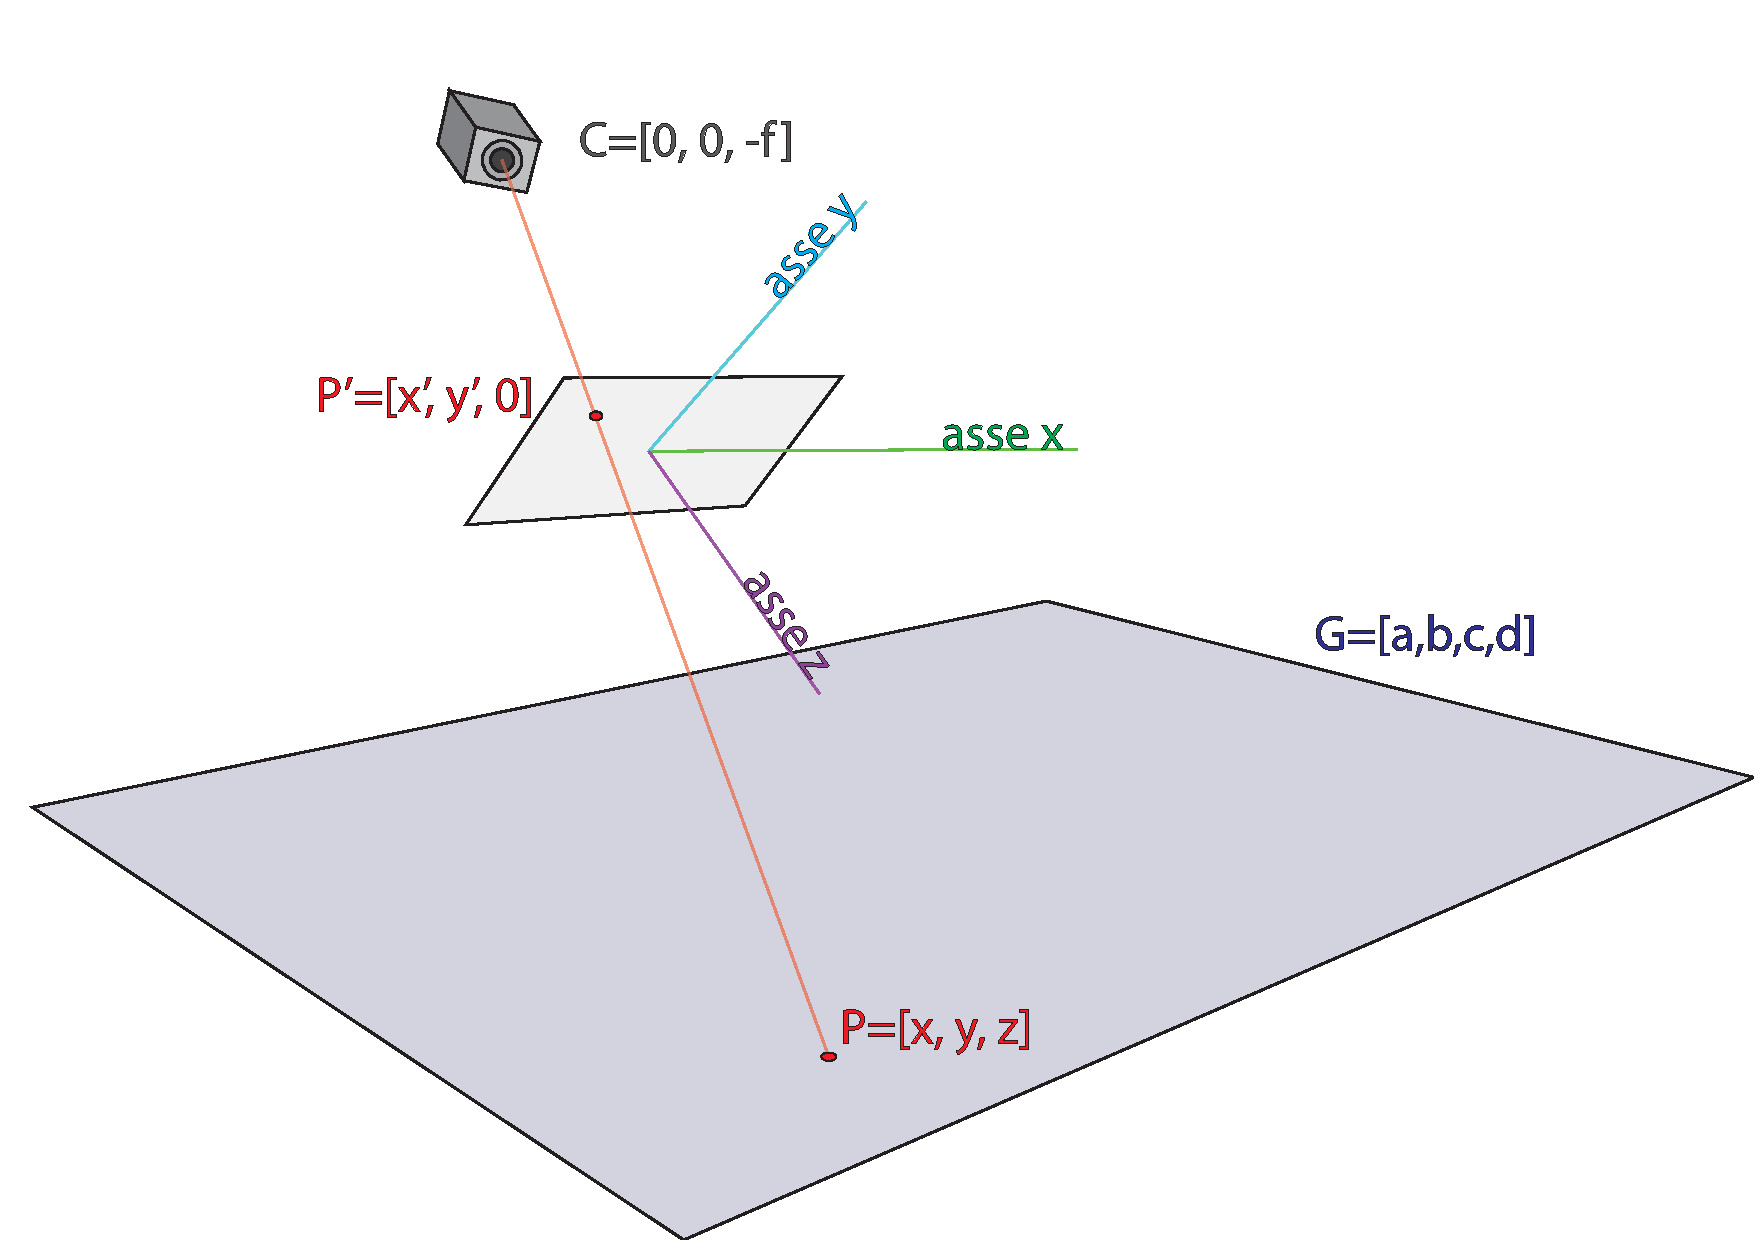
\includegraphics[width=\textwidth]{images/camera coords.pdf}
\end{figure}

È possibile definire tale matrice direttamente, ma è anche possibile definirla come combinazione di trasformazioni.
Tutte le trasformazioni affini sono componibili in coordinate omogenee, ed abbiamo quindi accesso a traslazione, rotazione e scalatura, a cui aggiungiamo la trasformazione di proiezione.
La trasformazione di proiezione prende le coordinate di un punto sull'immagine e, date le coordinate del piano, restituisce la posizione reale del punto corrispondente al punto immagine.
Dato che le coordinate sono omogenee e non cartesiane, il punto immagine è espresso con 3 coordinate e il punto reale trovato con 4 coordinate.
La trasformazione di proiezione è rappresentata con la matrice \ref{eq:projmat}:
\begin{equation}
    \label{eq:projmat}
    \begin{bmatrix}
        cf - d & 0      & 0   \\
        0      & cf - d & 0   \\
        -fa    & -fb    & -fd \\
        a      & b      & cf  \\
    \end{bmatrix}
\end{equation}
Dove:
\begin{itemize}
    \item il piano stradale è caratterizzato dall'equazione $ax + by + cz + d = 0$, oppure dal vettore $[a, b, c, d]^T$
    \item la lunghezza focale della camera è $f$
\end{itemize}

\textbf{TODO: bla bla spiega combinazione}
La matrice di trasformazione completa è definita quindi dalla combinazione di trasformazioni in \ref{eq:projcombo}:
\begin{equation}
    \label{eq:projcombo}
    \text{ \textbf{TODO}\  }
    M = C \cdot B \cdot A
\end{equation}
Dove:
\begin{itemize}
    \item blah
    \item blah blah
\end{itemize}
Ricordiamo che le trasformazioni combinano da destra verso sinistra.
Una rappresentazione visiva della combinazione è in fig \ref{fig:TODO}.

Diventa quindi possibile definire la matrice di correzione della distorsione prospettica in modo interattivo, manipolando la rotazione e la posizione della camera rispetto al piano stradale.
In questo modo si può trovare una trasformazione soddisfacente, in cui le misure si avvicinano a quelle reali, senza i grandi costi implementativi richiesti dall'implementazione di un metodo automatico per la definizione del piano stradale.
Una volta definita la matrice di trasformazione il suo utilizzo risulta estremamente efficiente, in quanto si riduce a un prodotto matrice-vettore.

L'ultima considerazione necessaria è la scelta del punto a cui applicare la trasformazione trovata.
Notiamo dall'immagine \ref{fig:TODO} che scegliere in punto centrale del Bounding Box non restituisce il risultato desiderato.
La strategia migliore è quella di proiettare il lato inferiore del Bounding Box, in quanto questo è l'unico che poggia sul piano stradale.
Il centro delle entità può poi essere approssimato date le conoscenze relative a dimensioni medie della sua tipologia, dalla sua direzione di movimento e dalle caratteristiche del Bounding Box.

In fig \ref{fig:TODO} è presentata una scena annotata dall'Object Detector Scaled-YoloV4.
In fig \ref{fig:TODO} è presentata la stessa scena dopo che è stata eseguita la correzione della distorsione prospettica, in cui la posizione dei veicoli è indicata dal cerchio verde.

\chapter{Correzione del rumore}
\label{sec:rumore}

\textbf{TODO}

\chapter{Architettura}
\label{sec:architettura}

\begin{figure}
    \centering
    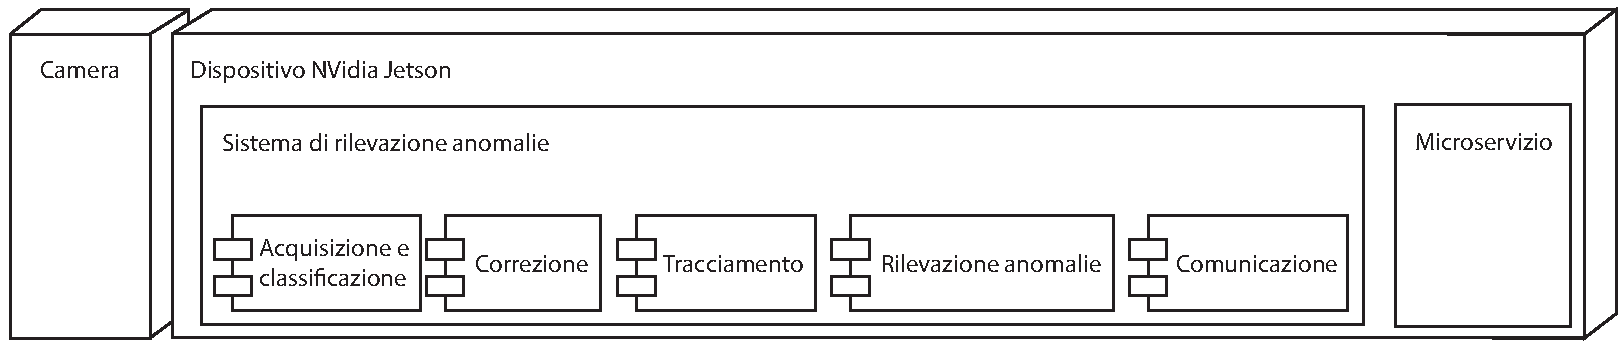
\includegraphics[width=\textwidth]{images/arch.png}
    \caption{Architettura del sistema}
\end{figure}

L'architettura scelta è una pipeline, in quanto l'input del sistema è uno stream video.
Ogni frame dello stream deve essere processato nello stesso modo, e utilizzare una pipeline consente di aggiungere, rimuovere o sostituire moduli, e quindi modificare il processo, in modo semplice e veloce.

Il sistema è implementato sul dispositivo \emph{Nvidia Jetson Xaxier}\cite{arch:jetson} ed è sviluppato su \emph{Ubuntu 18.04}\cite{arch:ubuntu}.
Il linguaggio di sviluppo è \emph{Python 3.6}\cite{arch:python}.
Per la gestione delle operazione di algebra lineare sono stati utilizzati i package \emph{Numpy}\cite{arch:numpy} e \emph{SciPy}\cite{arch:scipy}.
La pipeline di acquisizione è gestita dalla libreria \emph{GStreamer}\cite{arch:gstreamer}.
La classificazione è effettuata dal modulo di inferenza fornito dall'\emph{SDK Nvidia Deepstream}\cite{arch:deepstream}.
Questo modulo di inferenza è configurato per il modello di \emph{Object Detection Scaled--YoloV4}\cite{yolocsp}.
Il tracking è gestito dal tracker \emph{NvDCF} \cite{nvdcf}, anch'esso fornito dall'\emph{SDK Nvidia Deepstream}.
La segnalazione delle anomalie è effettuata utilizzando la libreria \emph{Requests} \cite{arch:requests}.

\chapter{Conclusioni}
\label{sec:conclusioni}

Abbiamo descritto un possibile approccio che permette di ricavare informazioni relative a posizione e velocità delle entità presenti nell'inquadratura di un sistema di sorveglianza stradale.
L'approccio descritto richiede che siano verificate varie condizioni, come per esempio che un piano sia una buona approssimazione del manto stradale e che l'intervallo di tempo tra una misura e l'altra sia piccolo e costante.
Nel caso questi non si verifichino nella nostra scena è possibile utilizzare soluzioni più sofisticate, come per esempio la Single View Metrology \cite{svm} per i problemi di prospettiva e Kalman Filter ed estensioni \cite{kalman} per i problemi di precisione nelle misure.

In questa tesi abbiamo lasciato alcune problematice aperte per quanto riguarda il posizionamento delle entità:
\begin{itemize}
    \item a seconda della direzione di movimento e della dimensione delle entità, l'approssimazione della posizione può essere più o meno buona.
    \item non è trattato un metodo per approssimare la forma delle entità, necessaria per lo sviluppo di un sistema in grado di rilevare urti tra di esse.
\end{itemize}
Queste problematiche rimangono al momento irrisolte.


\pagestyle{empty}

\chapter*{Ringraziamenti}
Ringrazio Salvatore, Silvio e Sebastian che mi hanno fatto trovare questo template pronto.


\addcontentsline{toc}{chapter}{Ringraziamenti}%

\bibliographystyle{splncs04}
\bibliography{bibliography}

\nocite{*}



% ----------------- ELENCO DELLE FIGURE/TABELLE ------------------------
\cleardoublepage
\listoffigures
\listoftables

\cleardoublepage


\end{document}
